\chapter{Introduction}

Kaggle is a platform owned by the Kaggle Inc. which is owned by Alphabet Inc. (Google) providing multiple so called challenges in the field of data science, predictive modeling and data analysis. The Kaggle challenge aims at solving so far unsolved tasks or finding a better solution for already solved tasks in a crowdsourcing fashion. Some challenges can be solved for monetary prices, others are hosted for knowledge or training purposes. In order to solve a challenge one must register and submit a solution to the platform to get a score for the submitted solution \cite{kaggle}.

The Google Landmark Recognition Challenge aims at detecting different landmarks in images, such as the Eiffel Tower or the Leaning Tower of Pisa \cite{challenge}.

We chose the Google Landmark Recognition Challenge because we are interested in image processing tasks and the challenge provides a lot of training data. We also wanted to try out Convolutional (Deep) Neural Networks which we previously discussed in the lecture.

The data provided with the challenge contains mainly of two CSV files. The file for training (train.csv) providing the IDs, URLs and Landmark IDs and the file for testing (test.csv) providing IDs and URLs \cite{data}.

In order to work with the images we wrote a script to scrape all URLs and download the images to our local machine. The script will be provided in the appendix.

Our approach is to first analyse the data to get a good understanding of it with the help of characteristic numerical values such as value ranges, min or max values and variances, which will be plotted for better visual understanding.

\chapter{Data Analysis}

Since the data provided with this challenge is contained purely out of images, we will focus on image-related characteristical numerical values for our analysis.

We selected the distribution of landmarks, the dimenions of the images, the amount of pixels, the pixel range (from min to max) and the pixel variance (max - min) to get a better understanding of what the images' shapes are.

The training dataset holds 1225029 URLs to images and the corresponding IDs and Landmark IDs. The five most frequent Landmark IDs are displayed in Figure \ref{landmark-ids} whith ID 9633 and ID 6051 being the most frequent ones. Figure \ref{9633} and \ref{6051} show images of the training dataset with these Landmark IDs.

The test dataset holds 117703 URLs to images with the corresponding IDs and will be purely used for validation of the trained model in Assignment 11.

\begin{figure}
	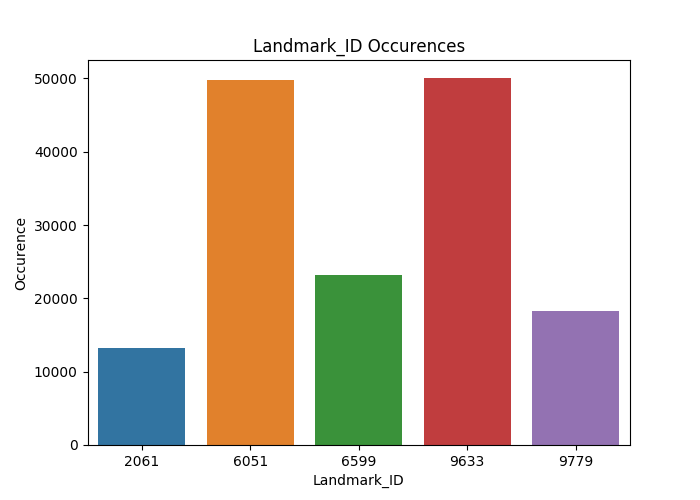
\includegraphics[width=\textwidth]{images/Landmark_ID_occurences}
	\label{landmark-ids}
\end{figure}
	
\begin{figure}
	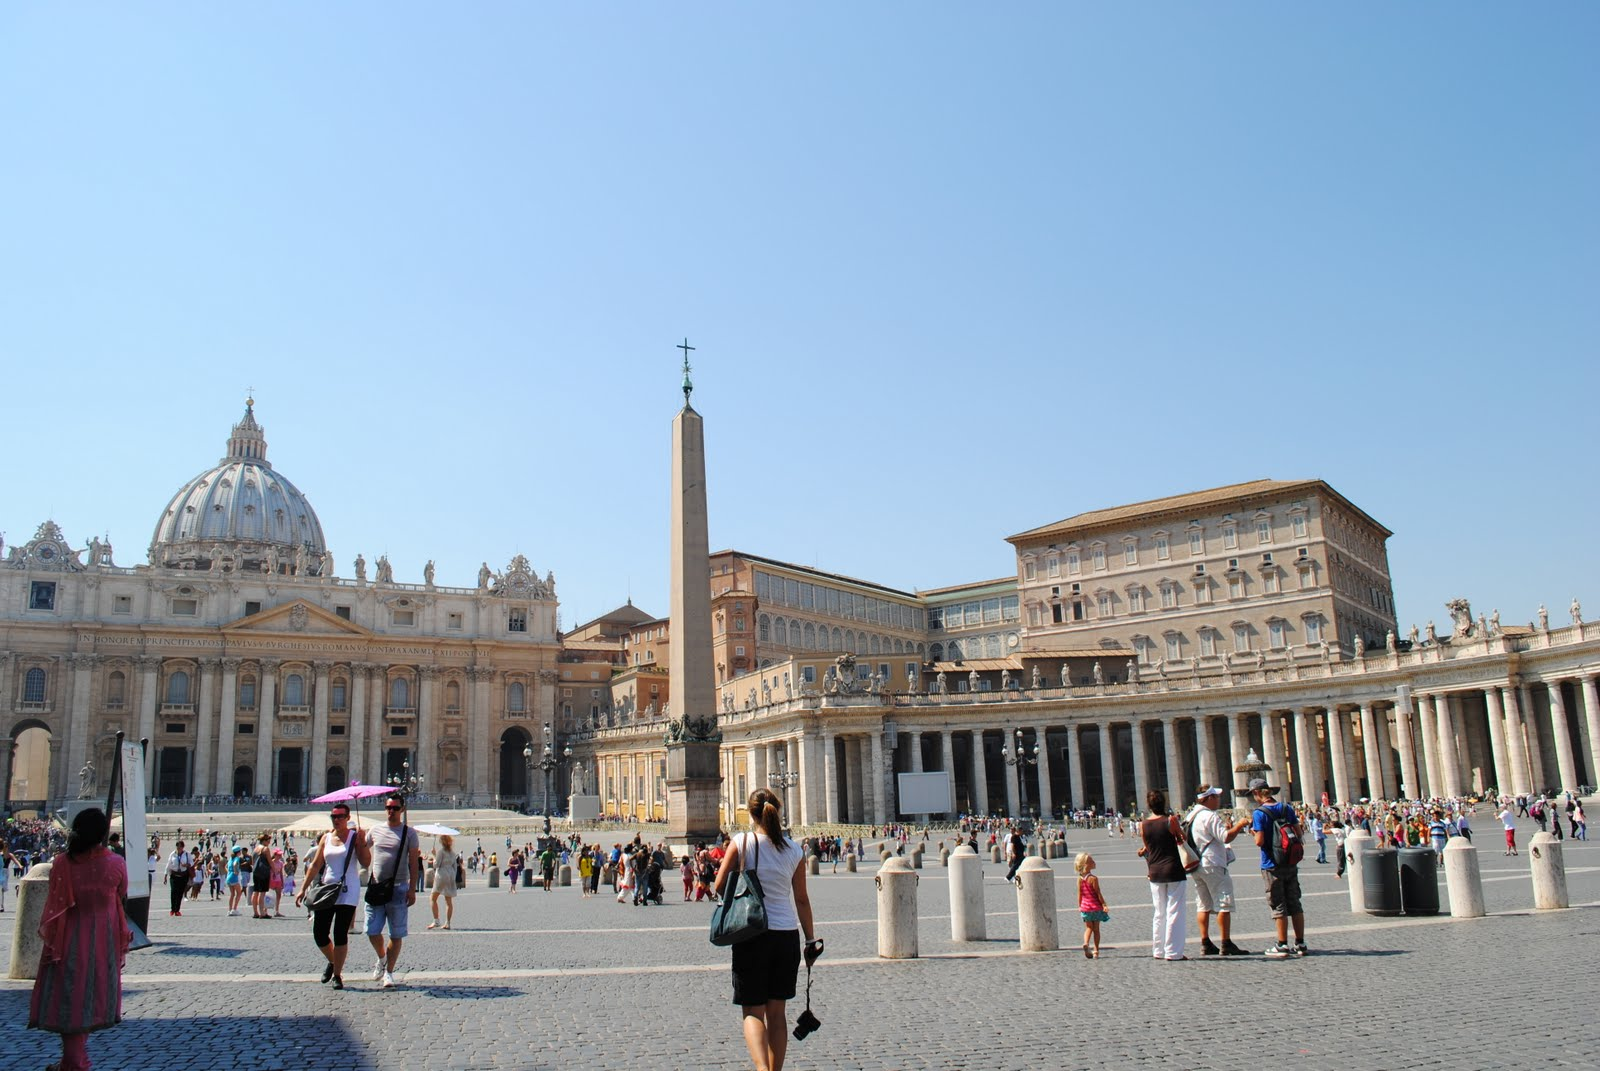
\includegraphics[width=\textwidth]{images/9633}
	\caption{Image for Landmark\_ID 9633}
	\label{9633}
\end{figure}
	
\begin{figure}
	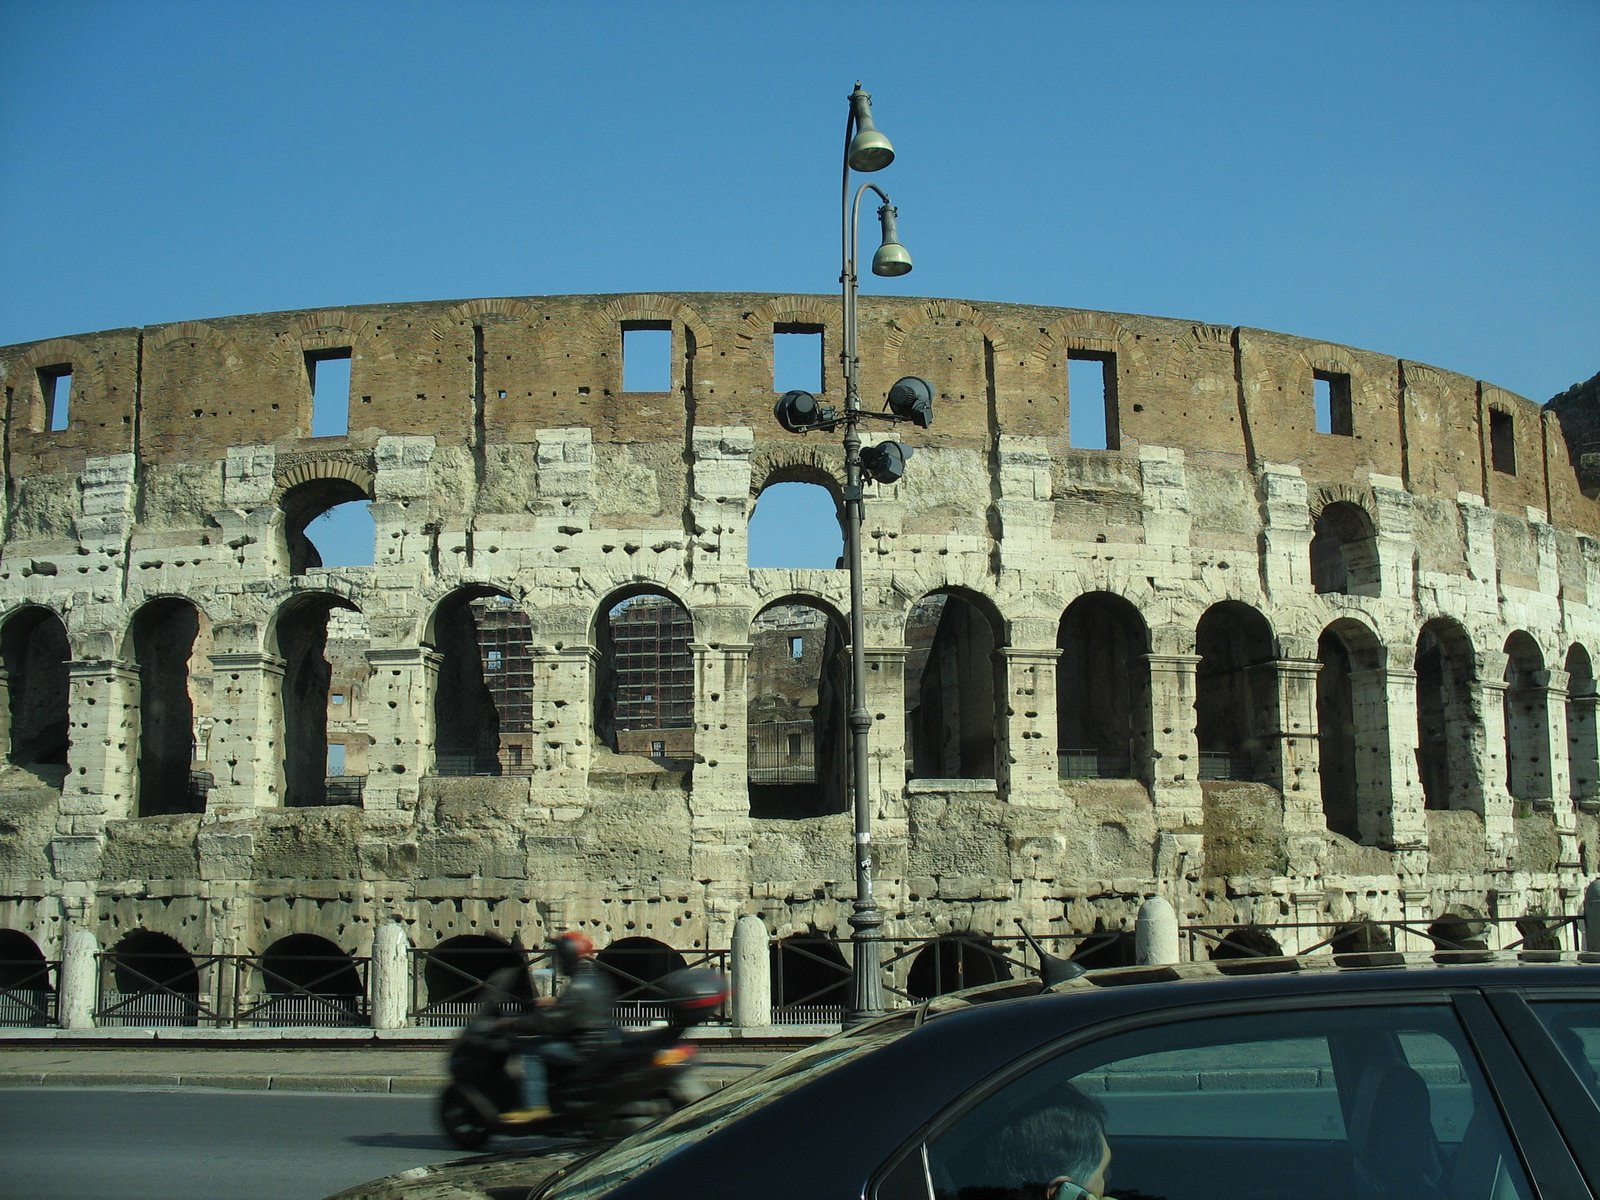
\includegraphics[width=\textwidth]{images/6051}
	\caption{Image for Landmark\_ID 6051}
	\label{6051}
\end{figure}

\begin{figure}
	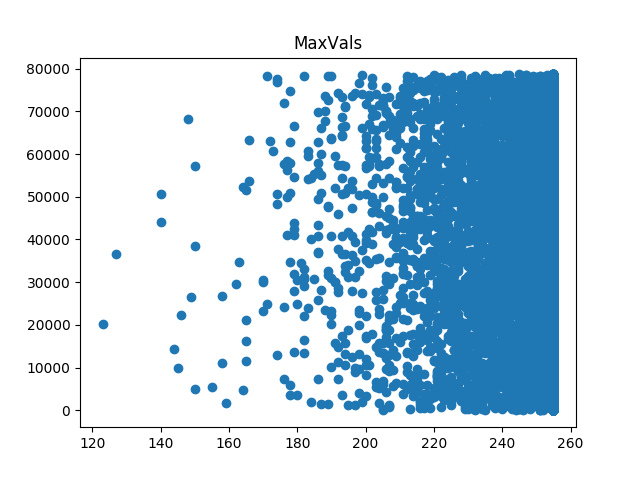
\includegraphics[width=\textwidth]{images/maxVals}
	\caption{maxVals}
	\label{maxVals}
\end{figure}

\begin{figure}
	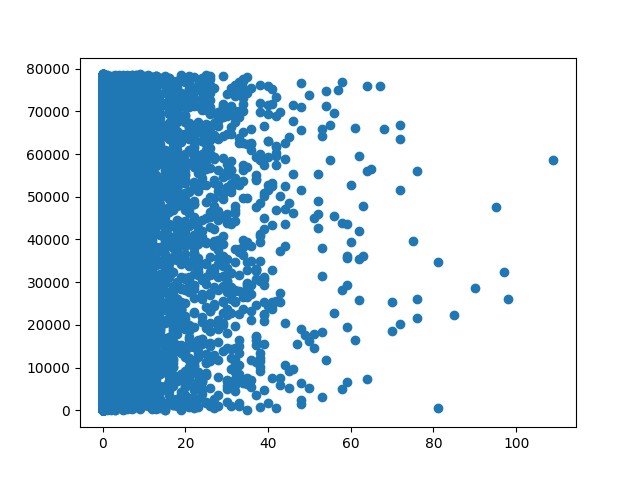
\includegraphics[width=\textwidth]{images/minVals}
	\caption{minVals}
	\label{minVals}
\end{figure}

\begin{figure}
	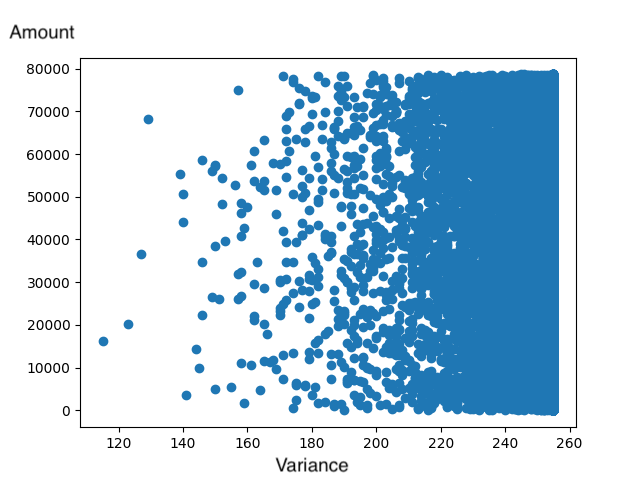
\includegraphics[width=\textwidth]{images/variances}
	\caption{Variances}
	\label{variances}
\end{figure}

\begin{figure}
	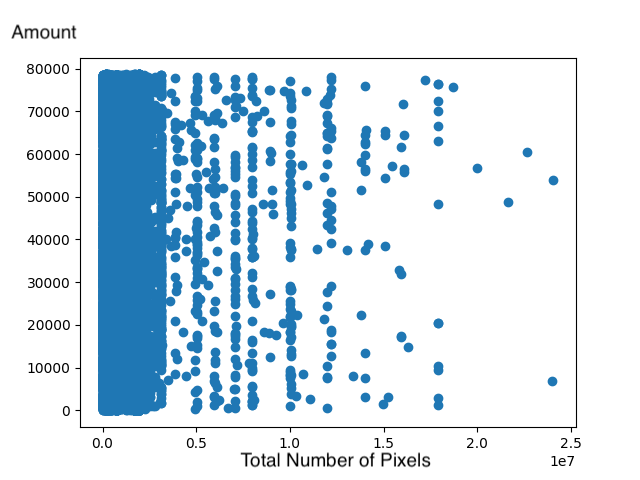
\includegraphics[width=\textwidth]{images/numPixels}
	\caption{numPixels}
	\label{numPixels}
\end{figure}

\begin{figure}
	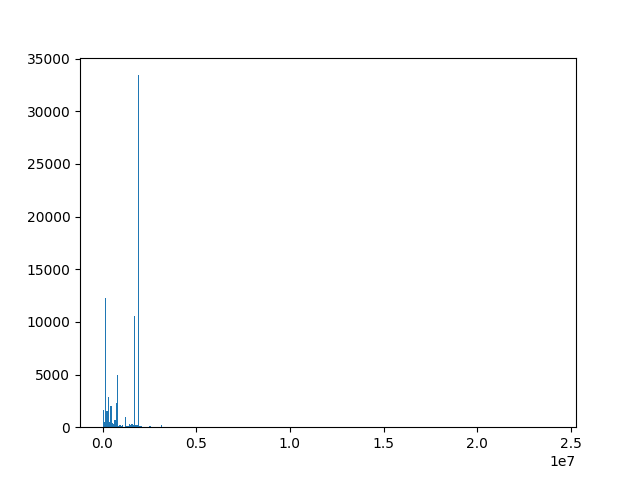
\includegraphics[width=\textwidth]{images/numPixelsHist}
	\caption{numPixelsHist}
	\label{numPixelsHist}
\end{figure}

imbalances, non-normalized features

extract features

are they correlated

cluster features with respect to correlation coefficient

which features are important

preprocess data

cluster data (or explain why not possible) (maybe cluster only some features)

dimensionality reduction method (e.g. PCA) or CNN Feature Map?

\section*{Interesting Features}
\section*{...}

\chapter{Conclusion}